\documentclass[a4paper,11pt,pdf]{pacmanreport}

%%=== Aditional packages
\usepackage{bm}
\usepackage{mhchem} % Package for chemical equation typesetting
\usepackage{siunitx} % Provides the \SI{}{} command for typesetting SI units
\usepackage{epstopdf}
\usepackage{booktabs}
\usepackage{floatrow}

\usepackage{amsmath}
\usepackage{amssymb}
\usepackage{colortbl}
\usepackage{gensymb}
\usepackage{algorithm}
\usepackage{algorithmic}

\usepackage{tikz}
\usetikzlibrary{shapes,arrows}
\usepackage{mathtools}
\usepackage{subcaption}

% The following is used to make packages hyperref and cite work together
\makeatletter
\let\NAT@parse\undefined
\makeatother
\usepackage[bookmarks=true,hyperfootnotes=true,colorlinks=true,linkcolor=blue,anchorcolor=blue,citecolor=blue,urlcolor=blue,filecolor=blue]{hyperref}

%%=== Local definitions
\graphicspath{{images/}{../shared_images/}{images/plots/}}

\newfloatcommand{capbtabbox}{table}[][\FBwidth]
%% ================================
%% PROJECT INFO 

\project{}
\projectid{FP7-IST-60918}
\projectstart{1 March 2013}
\duration{36}

%% ================================
%% MILESTONE INFO 

\title{Reactive haptic exploration control strategies ready for integration with planning}
\deliverableid{Milestone 4.2}
\author{M. Bonilla, C. Rosales, M. Gabiccini}
\address{Centro di Ricerca ``E. Piaggio'', Universit\`{a} di Pisa}
\email{manuel.bonilla@centropiaggio.unipi.t}
\headertitle{Exploration strategies}
\headerauthor{M. Bonilla, C. Rosales, M. Gabiccini}
\duedate{2015-02-28}
\submissiondate{2014-02-28}
\leadpartner{Universit\`{a} di Pisa}
\revision{draft}
\disseminationlevel{PU}

%% UNCOMMENT: to get the logo; if you've copied this file to a directory yearX/wpY/ then this should work
\reportlogo{pacmanlogo.png}

%% ======= Defining tikz style
\tikzstyle{block} = [draw, fill=blue!5, rectangle, 
    minimum height=3em, minimum width=6em]
\tikzstyle{block_small} = [draw, fill=blue!5, rectangle, 
    minimum height=3em, minimum width=3em]
\tikzstyle{sum} = [draw, fill=blue!5, circle]
\tikzstyle{intersection} = [fill,circle,minimum size=3pt,inner sep=0pt]
\tikzstyle{input} = [coordinate]
\tikzstyle{output} = [coordinate]
%%==============


\begin{document}

\maketitle

\begin{abstract}
\noindent This milestone details the work performed to integrate planning and execution phases involving object exploration and grasping. It aims to describe in detail the output of WP3, particularly the results of completing Task 3.1.
\end{abstract}


\vspace{.2em}
\hrule

\vspace{.2em}
\footnotesize

\tableofcontents

\normalsize

\newpage

\section{Milestone Summary and Context}

This milestone describes the work performed to integrate planning and execution phases concerning object exploration and grasping using a bimanual robot.

%The main contributions are 1) the technical implementation of hardware interfaces to command the KUKA LWR arm using ROS and 2)  the implementation of different classical controllers to move the robot using torque references.

%The first contribution is useful to command the robot using torque commands easier that using the actual KUKA FRI interface. The second helps to execute trajectories coming from planning phase, and to move the robot to desired references under different situations such as dynamic model uncertainty and different redundancy resolution at kinematic and dynamic levels. 

The platform presented in this milestone is of great importance within the PaCMan project the implementation, testing and validation of the development algorithms .


%In recent years, there has been growing interest in the development of a standardized framework for robotic implementations, where the robots interdisciplinary code and software could be easy to write and accessible to everyone. This is the philosophy of the \textit{Robot Operating System} (\textbf{ROS}), a flexible framework which provides all the instruments to develop and build robust and robot-independent applications, allowing researchers from different fields of robotics to share each others works with the great result of spreading the know-how.

Since ROS is the software framework used in PaCMan we developed a hardware interface for the robots used in the experimental platforms. However, this interface is just useful to command the robot using torque references. There are different strategies to generate the torque references to move a robot manipulator, they are designed for different situation for example under uncertainty, which main problem faced in PaCMan Project, in this case in the robot dynamics. Other strategies to deal with multi-goal references at kinematic and dynamic level were also implemented.

% What was the milestone that you are examining? What were the criteria for achieving it? What role does achievement of the milestone play in the whole project? How will its achievement as presented in this report contribute to the PaCMan scenarios and prototypes? 

% \subsection{Project Goals}

% The aim of this milestone report is focused on the development of a ROS-enabled software environment for controlling the manipulator KUKA LWR IV, used in the PaCMan platforms. 

After a first phase of studying and analyzing some of the novel approaches for robot control, the default control strategies provided by the manufacturer has been extended, implementing a new set of controllers.
The development of the controllers, including tuning and debugging, has been realized with the support of \textit{Gazebo}, a high performance realistic simulator which, interacting with ROS, gives the opportunity to test the efficiency of user-implemented control algorithms. 

%Finally, the last phase consisted in pursuing experiments to test the implemented control strategies on the physical robot, arising a variety of practical issues which don't come out in simulation, that are explained in detail in this document.

Controllers are available within the UNIPI \href{https://github.com/CentroEPiaggio/kuka-lwr}{KUKA LWR ROS package}, which is one of the components required by the Vito robot package freely available in the project website~\cite{PACMAN_software}. All packages within follow a dual implementation for real and simulated hardware, hence the same chosen controller can be tested in both scenarios with few or none extra-effort on the setup. Sec.~\ref{} describes Vito, the UNIPI robot as an alternative testbed for the project development.

\section{Report on Milestone Achievement}

%%% Learning the haptic characteristics of objects by exploration in-hand

\subsubsection{Learning the haptic characteristics of objects by exploration in-hand}
\label{sec:ControlAlgorithms}

This report used a fixture device as the supporting hand, and a 7 DOF robot as the exploratory finger. It is worth mentioning that a strategy for concurrent stable object grasping was demonstrated in DR5.1, and assumed to be given for the work presented here, and here we refer to the haptic exploration strategies only.

\paragraph{(a) Definition of control strategies for concurrent stable object grasping and object surface tracing for haptic exploration}

An Arimoto-PD regulator provides the required torques to track a reference position. The position control law is
\begin{equation}
    \bm{\tau_p} = G(\bm{q}) + K_{P_p} \left(\bm{\dot{q}_d}\Delta T\right) + K_{D_p}\bm{\dot{q}},
\end{equation}
where $G(\bm{q})$ is the gravity load vector, $\bm{{q}}$  is the generalized joint variables, $\bm{\dot{q}}$ is the measured rate of joints variables, $\Delta T$ the control period, and $K_{P_p}$,$K_{D_p}$ two positive definite matrices.

% \begin{figure}
% \begin{center}
% \includegraphics[width=0.65\textwidth]{finger_surface.png}
% \caption{Finger in contact with the unknown surface}
% \label{fig:finger_surface}
% \end{center}
% \end{figure}

A PID force controller is required to ensure contact during motion. The force control law is
\begin{equation}
    \bm{\tau_f} = f_dJ^T\bm{n_c} + K_{P_f}\bm{\tau_{e_n}} + K_{I_f}\int\bm{\tau_{e_n}}dt + K_{D_f}\dot{\bm{\tau}}_{e_n},
\end{equation}
where $J$ is the robot Jacobian matrix, $\bm{e_n} = (f_d - f_n)\bm{n_c}$ is the normal force error, $\bm{\tau_{e_n}} = J^T(\bm{q})\bm{e_n}$ is the normal force error in terms of joints torques, $\bm{v_d}$ the desired twist of the end effector, and $\bm{\dot{q}_d} = J^+\bm{v_d}$ the desired rate of angular joints.

Note that the position and force are to be controlled on the tangent plane and in the direction normal to it, hence due to their orthogonality, we can decouple the actions and sum up the contribution of each controller to form a hybrid force/position controller.

The strategy to slide a finger over a surface consist in assigning a reference velocity on the tangent plane at the contact point, of the same contact point. Let $C$ be the contact point and $\left\lbrace T \right\rbrace$ the frame with $C$ as origin, such that the $y$-$z$ directions form the local tangent plane and the $x$ direction is normal to the fingertip surface and pointing outwards, the desired twist of the fingertip with respect to $C$ written in $\left\lbrace T \right\rbrace$ is
\begin{equation}
    \bm{^Tv_C}=\left(
    \begin{matrix}
        0\\
        v_{dy}\\
        v_{dz}\\
        0\\
        0\\
        0
    \end{matrix}\right),
\end{equation}
where $v_{dy}$ and $v_{dz}$ are scalar components of the desired velocity in the local tangent plane, and $\sqrt{{v_{dy}}^2+{v_{dx}}^2}$ the norm of the assigned velocity. This is called the sliding primitive.

The desired twist of the fingertip center point, $P$, written in the end-effector frame $\left\lbrace E \right\rbrace$ is
\begin{equation}
\bm{^Ev_P}=\left(
    \begin{array}{cc}
       \bm{I}_{3x3} & ^E\hat{\bm{c}} \\
       \bm{0}_{3x3} & \bm{I}_{3x3}
    \end{array}
    \right)
    \left(
    \begin{array}{cc}
        R_{ET} & \bm{0}_{3x3} \\
        \bm{0}_{3x3} & R_{ET}
    \end{array}
    \right)
    \bm{{^Tv_C}},
\end{equation}
where $\bm{c}$ is a position vector from the fingertip center to the contact point, and the $\left(\hat{•}\right)$ operator is the skew-symmetric matrix extraction from a vector operator.

The Jacobian relative to the fingertip center is used to obtain the desired joint angle rates as
\begin{equation}
    \bm{\dot{q}_d}=J(\bm{q})\bm{^Ev_P}
\end{equation}

The set-point of the position controller is the updated joint angles
\begin{equation}
    \bm{q_d}=\bm{\dot{q}_d}\Delta_T+\bm{q},
\label{anglejointsreference}
\end{equation}
where $\Delta_T$ is the control period.

%% THE PPC CONTROLLER, NOT SURE TO INCLUDE IT

% A more general class of the adaptive controllers called Prescribed Performance Controller (PPC) proposed by~\cite{DoulgeriPPC} achieves force/position tracking with prescribed performance and ensures no loss of contact with the surface under parametric uncertainties in robot dynamics and contact compliance. Prescribed performance is presented in terms of convergence rate, steady state error and allowed overshoot for the force/position tracking errors.

% The strong limitation of such controller is that it \textbf{is derivated only for a fixed planar surface}; the robustness by utilizing the controller to perform the same task of the Hybrid F/P one is a possible subject of a future work. Altough a complete mathematical derivation of the controller is in ~\cite{DoulgeriPPC}, here the necessary for the implementation is presented.

% Let the base frame be {B}. Let the surface frame be {S} and attached at some point on the surface; its position is denoted by a vector $\bm{p_s} \in R^3$ and its orientation by a matrix $R_s =[\bm{n_s, o_s, a_s}]$, such that $\bm{n_s} \in R^3$ is the unit vector normal to the contact surface pointing inwards.

% Consider also the end effector frame ${\mathcal{E}}$ described by a position vector $\bm{p_t} \in R^3$ and an orientation matrix $R_t$ that can be parameterized by three rotation angles around the axes of the inertia frame, denoted by $\bm{\phi_t} \in R^3$. Let the generalized position be $\bm{p} = [\bm{p_t^T, \phi_t^T}]^T \in R^6$. The generalized velocity $\dot{\bm{p}} = [\dot{\bm{p}}_t^T, \bm{\omega}_t^T]^T$ is related to the joint velocity $\bm{\dot{q}}$ through the robot Jacobian
% \begin{equation}
%   \dot{\bm{p}}=J(\bm{q})\dot{\bm{q}}.
% \end{equation}

% Assume that the position and orientation of the surface is known and hence $\bm{n_s}$ and the generalized normal vector $\bm{n} = [\bm{n^T , 0_3^T}]^T$ can be used to calculate projection matrices $Q_s =[ I_{3 \times 3} - \bm{n_sn_s^T}]$, $Q=[I_{6 \times 6} - \bm{nn^T}]$ to the position/orientation subspace.

% For a planar surface it is possible to derive the material deformation $\chi$ as a function of $\bm{p_s}$ and $\bm{p}$:
% \begin{equation}
%   \chi = r- \bm{n_s^Tp_s+n_s^Tp_t},
% \end{equation}
% and its derivative:
% \begin{equation}
%   \dot{\chi}=\bm{n^T}\dot{\bm{p}}=\bm{n_s^T}\dot{\bm{p_t}},
% \end{equation}
% where a semispherical end effector of radius $r$ is assumed. As the robot interacts with the surface, an interaction wrench $\bm{w} \in R^6$ arises from the contact, that is measured by a force/torque sensor. This force includes both normal $\bm{n}f$ and tangential forces and torques $Q\bm{w}$.

% Assume that the normal force magnitude $f$ is in general a positive monotonically increasing continuously differentiable nonlinear function of the deformation $\chi$, say
% \begin{equation}
% \bar{f}=\begin{cases}
% f(\chi),\, \chi \ge 0\\
% 0,\, \chi <\ 0.
% \end{cases}
% \end{equation}
% We further assume that the \textbf{force deformation relationship} $f(\chi)$ can be modeled by a \textbf{weighted sum of positive powers of the deformation} $\chi$, that is
% \begin{equation}
% f(\chi)=Z_f^T(\chi)\theta_f,
% \end{equation}
% with
% \begin{equation}
% Z_f(\chi)=[\chi^{\mu_1} \ldots \chi^{\mu_{n_f}}], \; \mu_i \in R^+,
% \end{equation}
% and
% \begin{equation}
% \theta_f=[\theta_{f_1} \ldots \theta_{f_2}].
% \end{equation}

% Define also a quantity that will be useful below:

% \begin{equation}
% \vartheta Z_f = \frac{\partial Z_f(\chi)}{\partial \chi}
% \end{equation}

% In a force/position tracking problem the robot end effector is desired to track a force trajectory $\bm{n}f_d(t)$ along the normal to the surface direction and a desired position trajectory $Q_s\bm{p}_{\bm{t}d}(t)$ on the surface. The desired position trajectory $\bm{p}_{\bm{t}d}(t)$ may be defined in local surface coordinates as $\bm{\xi}_{d}(t)=[\xi_{d_1}(t), \xi_{d_2}(t)]^T \in R^2$ and $\bm{p}_{\bm{t}d}(t)$ is then calculated using information on surface position and orientation: $\bm{p}_{\bm{t}d}(t)=R_s[0, \bm{\xi}_{d}^T(t)]^T+\bm{p_s}$. Define also a orientation trajectory $\bm{\phi}_{td}$ an obtain the desired generalized position
% \begin{equation}
%   \bm{p}_d(t)=[\bm{p}_{\bm{t}d}^T(t) \bm{\phi}_{\bm{t}d}^T(t)].
% \end{equation}

% The control objective of PPC is twofold: 1) track the desired generalized position trajectory $Q\bm{p}_d(t)$ on the surface and 2) track the desired force trajectory $\bm{n}f_d(t)$ normal to the surface in presence of parametric uncertainties in the robot dynamics and the force deformation model, while keeping all signals in the closed loop bounded.

% The meaning of prescribed performance is that the position error $\bm{e}_p = Q(\bm{p}-\bm{p}_d)$ and the normal force error $e_f=(f-f_d)$ evolve within a predefined region that is bounded by a decaying function of time. Assuming an error
% signal $e(t)$, ($e(t)$ may be $\bm{e}_p(t)$ or $e_f(t)$), the mathematical expression of prescribed performance is given,
% for $t\ge0$, by the following inequalities
% \begin{equation}
%   \begin{cases}
%       -M\rho(t) <\ e(t) <\ \rho(t),\, e(0) >\ 0\\
%       -\rho(t) <\ e(t) <\ M\rho(t),\, e(0) <\ 0,
%   \end{cases}
% \end{equation}
% with $-1 <\ M <\ 1$ and $\rho(t)$ is a bounded, smooth, strictly positive, decreasing function with $\lim_{t \to \infty}\rho(t)= \rho_\infty >\ 0$. A possible choose for $\rho(t)$ is
% \begin{equation}
%   \rho(t)=(\rho_0-\rho_\infty)\exp(-lt),
% \end{equation}
% with $\rho_0 >\ |e(0)|$, and $\rho_\infty$ representing the maximum permissible size of the tracking error at steady state. The satisfaction of performance bounds for the force error allows us further to guarantee that the robot will never lose the contact with the surface.

% To satisfy both control objectives define the error trasformation
% \begin{equation}
%   \epsilon(t)=T\left(\frac{e(t)}{\rho(t)}\right),
% \end{equation}
% with
% \begin{equation}
% T(x)=\begin{cases}
%   \log\left(\frac{M+x}{1-x}\right),\, e(0) >\ 0\\
%   \log\left(\frac{1+x}{M-x}\right),\, e(0) <\ 0
%   \end{cases}
% \end{equation}

% In this way the satisfaction of the prescribed performance is obtained simply by keeping $\epsilon(t)$ bounded. Thus, let
% \begin{equation}
% \epsilon_f(t)=T_f\left(\frac{e_f(t)}{\rho_f(t)}\right),
% \end{equation}
% \begin{equation}
% {\bm{\epsilon}_p}(t)=\bm{T}_p\left(\frac{{\bm{e}_p}(t)}{{\bm{\rho}_p}(t)}\right),
% \end{equation}
% \begin{equation}
% \vartheta T_f=\frac{\partial T_f}{\partial \left( \frac{e_f}{\rho_f}\right)}\frac{1}{\rho_f},
% \end{equation}
% and
% \begin{equation}
% \vartheta \bm{T}_p=\frac{\partial \bm{T}_p}{\partial \left( \frac{\bm{e}_p}{\bm{\rho}_p}\right)}\frac{1}{\bm{\rho}_p}.
% \end{equation}
% Consider the following reference velocity vector $\dot{\bm{p_r}}$ in the robot tip operational space
% \begin{equation}
%   \dot{\bm{p_r}}=\bm{n}\frac{\dot{f_d}+\frac{\dot{\rho_f}}{\rho_f}\left(Z_f^T\hat{\bm{\theta}}_f-f_d\right)}{\vartheta Z_f^T\hat{\bm{\theta}}_f}+Q\left(\dot{\bm{p_d}}+\frac{\dot{\bm{\rho}_p}}{\bm{\rho}_p}\bm{e}_p\right),
% \end{equation}
% the proposed control law is
% \begin{equation}
%   u=-k_fJ^T\bm{n}\vartheta Z_f^T\hat{\bm{\theta}}_f\vartheta T_f\epsilon_f-k_pJ^TQ\vartheta \bm{T}_p\bm{\epsilon}_p+Z_d^T(\bm{q,\dot{q},\dot{q}_r,\ddot{{q}}_r})\bm{\hat{\theta}}_d+J^T\bm{w}-D\bm{s_q},
% \end{equation}
% where
% \begin{equation}
%   \bm{\dot{q}}_r=J^+\dot{\bm{p_r}}
% \end{equation}
% and
% \begin{equation}
%   \bm{s_q}=\dot{\bm{q}}-\dot{\bm{q_r}}.
% \end{equation}
% Furthermore, we have indicated with $Z_d^T(\bm{q,\dot{q},\dot{q}_r,{\ddot{q}}_r})$ the Slotine Lie regressor of the manipulator. Moreover, $k_f$, $k_p$ are positive scalar control gains and $D$ is a positive definite matrix.

% Note that, $\bm{\hat{\theta}}_f$ and $\bm{\hat{\theta}}_d$ used in the above equations are respectively the estimation of the unknown parameters vectors $\bm{{\theta}}_f$ and $\bm{{\theta}}_d$ provided by the update laws
% \begin{equation}
%   \dot{\bm{\hat{\theta}}}_f=P_f\left\lbrace \Gamma_fk_f\epsilon_f\vartheta T_f\left(\vartheta Z_f\dot{\chi}-\frac{\dot{\rho}_f}{\rho_f}Z_f\right)\right\rbrace
% \end{equation}
% and
% \begin{equation}
%   \dot{\bm{\hat{\theta}}}_d=-\Gamma_dZ_d^T(\bm{q,\dot{q},\dot{q}_r,\ddot{{q}}_r})\bm{s_q},
% \end{equation}
% with $\Gamma_f$ and $\Gamma_d$ positive definite matrices.

\paragraph{(b) Definition of control strategies for concurrent stable object grasping and rolling manipulation to acquire second-order object surface properties}

Based on the previous control framework, rolling over a surface is achieved by defining a reference velocity of the contact point for a pure revolution about an axis laying on the tangent plane and passing through the contact point. Similar to the previous section, the desired twist of the contact point $C$ written with respect to $\left\lbrace T \right\rbrace$ is
\begin{equation}
    \bm{^Tv_C}=\left(
    \begin{array}{c}
        0\\
        0\\
        0\\
        0\\
        \omega_{dy}\\
        \omega_{dz}\\
    \end{array}\right),
\end{equation}
where $\omega_{dy}$ and $\omega_{dz}$ are the scalar components of the desired rolling velocity, and $\sqrt{{\omega_{dy}}^2+{\omega_{dx}}^2}$ is the norm of the assigned velocity. This is called the rolling primitve.

The desired twist of the fingertip center and the desired joint angle rates rate of joint angles are obtained as in the previous paragraph.

To estimate the curvature of the unknown surface, which is a second-order property, it is possible to use Montata's equations for two object in pure rolling contact, namely
\begin{equation}
M_f \dot{\alpha}_f=(K_f+\tilde{K}_0)^{-1}
\left[
\begin{array}{c}
-\omega_y\\
\omega_x\\
\end{array}
\right],
\label{eq:montana}
\end{equation}
where $\dot{\alpha}_f$ is the velocity of the contact point in the local surface chart (measured), $M_f$ is the metric form of the fingertip surface (known), $K_f$ is the curvature form of the fingertip surface (known), $\omega_x$ and $\omega_y$] are the rolling component of the relative angular velocity of the Gauss frame (measured), and $\tilde{K}_0$ is the curvature form of the object surface (estimated).

For a finite rolling motion, it is possible to approximate (\ref{eq:montana}) with
\begin{equation}
M_f \Delta{\alpha}_f=\bar{K}_r
\left[
\begin{array}{c}
-\Delta\theta_y\\
\Delta\theta_x\\
\end{array}
\right],
\label{montanaapprox}
\end{equation}
where
\begin{equation}
\bar{K}_r=(K_f+\tilde{K}_0)^{-1}=
\left(
\begin{array}{cc}
r_1 & r_2 \\
r_2 & r_3
\end{array}
\right),
\end{equation}
or equivalently,
\begin{equation}
    \bm{b}=A\bm{r},
\end{equation}
with
\begin{equation}
    \bm{b}=M_f \Delta{\alpha}_f,
\end{equation}
\begin{equation}
A=\left(
\begin{array}{ccc}
-\Delta\theta_y & \Delta\theta_x & 0\\
0 & -\Delta\theta_y & \Delta\theta_x\\
\end{array}
\right),
\end{equation}
and
\begin{equation}
\bm{r}=\left(
\begin{array}{c}
r_1\\
r_2\\
r_3
\end{array}
\right).
\end{equation}

Therefore, using the generalized inverse as
\begin{equation}
\bm{r}=A^+\bm{b},
\end{equation}
it is possible to estimate the curvature form of the object surface,
\begin{equation}
\tilde{K}_0=\bar{K}_r^{-1}-K_f,
\end{equation}
and by diagonalization,
\begin{equation}
K_0=R^T(\psi)\tilde{K}_0 R(\psi)
\end{equation}
obtain the principal curvature directions given by $\psi$, and principal curvatures at the contact point, $\tilde{K}_0$.

% \section{Quadric model}
% To estimate the unknown surface a quadric model can be assumed:
% \begin{equation}
% S(\bm{r})=\bm{r^TQr+2p^Tr}-k=0
% \end{equation}

% and the normal surface is described by:
% \begin{equation}
% \nabla_r^TS(\bm{c})=2\bm{Qr}+2\bm{p}
% \end{equation}

% where $Q \in R^{3 \times 3}$ and symmetric, $\bm{p} \in R^3$ and $\bm{r} \in R^3$ position vector of the object surface.
% At each contacted point $(c,n_c)$ holds
% \begin{equation}
% \begin{cases}
% S(\bm{c})=0\\
% \nabla_r^TS(\bm{c})+k\bm{n_c}=0
% \end{cases}
% \end{equation}

% From the previuos system of equation holds
% \begin{equation}
% \bm{y=Wa}
% \end{equation}

% with

% \begin{equation}
% \bm{a}=[q_{11}, q_{22}, q_{33}, q_{12}, q_{23}, q_{13}, p_1, p_2, p_3, k]^T
% \end{equation}

% \begin{equation}
% \bm{W}=\left(
% \begin{matrix}
% x^2 & y^2 & z^2 & 2xy & 2yz & 2xz & 2x & 2y & 2z & 0 \\
% x & 0 & 0 & y & 0 & z & 1 & 0 & 0 & n_x\\
% 0 & y & 0 & x & z & 0 & 0 & 1 & 0 & n_y\\
% 0 & 0 & z & 0 & y & x & 0 & 0 & 1 & n_z
% \end{matrix}
% \right)
% \end{equation}

% \begin{equation}
% \bm{y}=[1,0,0,0]^T
% \end{equation}

% The estimation can be made in batch processing. After N contact points have been registered, solve:

% \begin{equation}
% \bm{a}=\bar{\bm{W}}^+\bar{\bm{y}}
% \end{equation}

% with $\bar{\bm{W}} \in R^{4N \times 10}$ and $\bar{\bm{y}} \in R^{4N}$

\paragraph{(c) Definition of strategies for frictional coefficient estimation}
Using the strategy described in paragraph (a), one can compensate for the tangential force generated due to the frictional property of the object. The tangential force can be extracted from the measured contact force as
\begin{equation}
    \mathbf{f}_t = (I-\mathbf{n}_{c}\mathbf{n}^T_{c})\mathbf{f}_c,
\end{equation}
and the dynamic friction coefficient at the contact point can be readily obtained as
\begin{equation}
    \mu_{d} = \lVert{\mathbf{f}_{t}}\rVert/\lVert{\mathbf{f}_{n}}\rVert.
\end{equation}

Knowing the fingertip material and using a usal look-up table fo friction coefficients, one can query by the pair material-dynamic coefficient, and thus obtain the static coefficient, as a well as the object material.

Finally, the compensation will be achieved by adding the term
\begin{equation}
    \boldsymbol{\tau}_f=-J^T \mathbf{f}_t,
\end{equation}
to the force controller.

\paragraph{(d) Testing in simulation}
The simulation framework is heavily based on Adams MSC\copyright, a software for multi-body dynamic simulation and collision management. It uses several contact models based on a penalty formulation on the inter-penetration between meshes. The geometry engine is responsible for detecting contact between two geometries, locating the points of contact, and calculating the common normal at the contact points. Once the contact kinematics are known, contact forces, which are a function of the contact kinematics, are applied to the intersecting bodies. The model adopted is a Hertzian model, named \emph{Impact} by Adams (see Fig.~\ref{fig:contactedmesh}).

Another feature is the capability to export a Simulink block representing the articulated model with inputs (e.g. joint torques) and outputs (e.g. joint angles, contact wrench). Matlab and Simulink were used to implement the control laws and to manage the results.

Thus, a planar finger with three angular joints was modeled using the parameters in Table~\ref{tab:3R}. The fingertip is a hemisphere of radius $3$ cm.

\begin{table}
\centering
\begin{tabular}{cccccccc}
    \toprule
    \textbf{joint} & $\theta$ & $d$ [m] & $a$ [m] & $\alpha$ & \textbf{Mass [Kg]} & $I_{zz}$ [Kgm] & \textbf{CoG [m]}\\
    \toprule
    1 & $q_1$ & $0$ & $0.05$ & 0 & $0.02$ & $5e^{-6}$ & $(0, -0.0250, 0)^{T}$\\
    \midrule
    2 & $q_2$ & $0$ & $0.05$ & $0$ & $0.02$ & $5e^{-6}$ & $(0, -0.0250, 0)^{T}$\\
    \midrule
    3 & $q_3$ & $0$ & $0.05$ & $0$ & $0.02$ & $5e^{-6}$ & $(0 -0.0250 0)^{T}$\\
    \bottomrule
\end{tabular}
\caption{DH and dynamic parameters of the 3R finger.}
\label{tab:3R}
\end{table}

The controller gains for position and force regulation and contact parameters between the fingertip and the objects were set as in Table~\ref{tab:sim_parameters}. The desired normal component contact force was set to $1$N for all cases.

\begin{figure}
\begin{floatrow}
\ffigbox{%
  \includegraphics[width=\linewidth]{contacted_mesh.png}%
}{%
\caption{Contact model in Adams.}%
\label{fig:contactedmesh}%
}
\capbtabbox{%
    \begin{tabular}{cccc}
    \toprule
    \textbf{Parameter} & \textbf{Value}\\
    \toprule
    $K_{P_p};K_{D_p}$ & $100;20$\\
    \midrule
    $K_{P_f};K_{D_f};K_{I_f}$ & $10;1;0.1$\\
    \midrule
    Stiffness & 1000$\frac{N}{m}$\\
    \midrule
    Damping & 20$\frac{Ns}{m}$\\
    \bottomrule
    \end{tabular}
}{%
    \caption{Test parameters.}%
    \label{tab:sim_parameters}%
}
\end{floatrow}
\end{figure}


Fig.~\ref{fig:NormCompContForce} shows the track of the normal component of the contact force for the sliding on a plane and a sphere surface. And Fig.~\ref{fig:TangCompForce} shows the track of the normal and tangential force during rolling over the a plane.

\begin{figure}[!t]
\centering
\mbox{
\includegraphics[width=0.45\linewidth]{NormalComponentContactForcePLANE.png}
\includegraphics[width=0.45\linewidth]{NormalComponentContactForceSPHERE.png}
}
\caption{Normal component of the contact force when sliding over a plane (left) and a sphere (right).}
\label{fig:NormCompContForce}
\end{figure}

\begin{figure}[!t]
\centering
\mbox{
\includegraphics[width=0.45\linewidth]{NormalComponentContactForceROLLPLANE.png}
\includegraphics[width=0.45\linewidth]{TangentialComponentContactForceROLLPLANE.png}
}
\caption{Normal (left) and tangential (right) component of the contact force when rolling over a plane.}
\label{fig:TangCompForce}
\end{figure}

The tests were taken to a real scenario shown in Fig.~\ref{fig:curvature}, where the KUKA LWR was equipped with an ATI Nano 17 force torque sensor. The estimated principal curvatures are summarized in Table~\ref{tab:results}. Note that the sphere is a basketball, whose official radius is 11,92-12,07cm, as well as the large values for the plane and one of the pricnipal curvatures on the cylinder.

\begin{table}
\centering
\caption{Experimental Results}
\label{tab:results}
\begin{tabular}{ccccc}
    \toprule
    & \multicolumn{4}{c}{\textbf{Princial Radii}}\\
    \textbf{Object} & \multicolumn{2}{c}{\textbf{Real}} & \multicolumn{2}{c}{\textbf{Estimated}}\\
    \textbf{Direction} & $z$ [m] & $y$ [m] & $z$ [m] & $y$ [m]\\
    \toprule
    Plane & $\infty$ & $\infty$ & 333 & 500 \\
    Cylinder & $\infty$ & .90 & 500 & .088 \\
    Sphere & .1207 & .1207 & 0.121 & 0.127 \\
    \bottomrule
\end{tabular}
\end{table}

\begin{figure}[!h]
    \centering
    \label{fig:curvature}
    \mbox{
    \includegraphics[width=.33\linewidth]{plane}
    \includegraphics[width=.33\linewidth]{cylinder}
    \includegraphics[width=.33\linewidth]{basketball}
    }
    \caption{Test objects for curvature estimation test on a plane (left), a cylinder (middle), and a sphere (right).}
    \vspace{9pt}
\end{figure}


%This results will be tested again in the new simulation framework presented in~\ref{sec:Simulation}.

\paragraph{(e) Integration of object/part model obtained from vision with the code for reactive haptic exploration strategies}

\begin{figure}[!b]
  \begin{center}
    \includegraphics[width=1.0\linewidth]{sliding}
  \end{center}
  \caption{The shape is acquired by an RGBD sensor and the friction coefficients by the intrinsic tactile sensor, both shape~$f(\mathbf{x})$ and friction~$m(\mathbf{x})$ functions are represented as a Gaussian Process $\mathcal{GP}(0,k(\cdot))$. The exploration follows geodesic flows~$\gamma_i$ on the surface of a fixed object using a compliant behavior.}
  \label{fig:schema}
\end{figure}

The setup overview is depicted in Fig.~\ref{fig:schema}. The approach used Gaussian Processes to represent both shape and fiction coefficient. This representation was successfully exploited to generate exploratory trajectories on the object surface, even with arbitrary shapes. The normal contact force was used to distinguish between the contact and the non-contact states. The exploratory probe was the same as in the previous paragraph, with an additional compliant coupler for safety and sensor protection. Only sliding controller was used since the friction coefficient is simpler to retrive using that primitive. More details on the methodology can be found in the attached paper~\cite{Active2014Rosales} available at~\href{./attachedPapers/ActiveGatheringOfFrictionalPropertiesFromObjects.pdf}{this link}.

% \begin{figure}[th]
%     \centering
%     \mbox{
%         \includegraphics[height=0.4\linewidth]{box.png}
%         \includegraphics[height=0.4\linewidth]{box1.png}
%         }
%     \mbox{
%         \includegraphics[height=0.4\linewidth]{teddy.png}
%         \includegraphics[height=0.4\linewidth]{teddy2.png}
%         }

%     \caption{Geodesic flows on object surfaces captured by an RGBD sensor. The color of the flow goes from red, i.e. the initial contact point, to green, i.e. the final position, according to the predefined length of the curve. The box has flat surfaces, hence geodesics are straight lines (top). The teddy bear has a very irregular shape, but still geodesic flows are found (bottom).}
%     \label{fig:geodesic_examples}
%     \vspace{-0.02\linewidth}
% \end{figure}

% \begin{figure}
%   \centering
%   \mbox{
%         \includegraphics[width=0.45\linewidth]{FZBOX.png}
%         \includegraphics[width=0.45\linewidth]{MuBOX.png}
%         }
%     \caption{Relevant data recorded during a haptic exploration. Force along $\mathbf{z}_{\text{c}}$ used to detect the contact and non-contact states (top). Friction coefficient $\mu$, the red line marks the mean value during the contact state (bottom). Material: Paperboard.}
%     \label{fig:data2}
% \end{figure} 

\newpage

\bibliographystyle{IEEEtran}
\bibliography{../shared_bibliography/abbreviations,bibliography/MS42}

\newpage
\appendix
\section{Annexes}

% Here you should briefly describe the papers attached that provide evidence for achievement of the milestone. Mention titles, authors, publication info; abstract; and a one-liner relating the publication back to the discussion on actual work performed. 

%% ======= Defining tikz style
\tikzstyle{block} = [draw, fill=blue!5, rectangle, 
    minimum height=3em, minimum width=6em]
\tikzstyle{block_small} = [draw, fill=blue!5, rectangle, 
    minimum height=3em, minimum width=3em]
\tikzstyle{sum} = [draw, fill=blue!5, circle]
\tikzstyle{intersection} = [fill,circle,minimum size=3pt,inner sep=0pt]
\tikzstyle{input} = [coordinate]
\tikzstyle{output} = [coordinate]
%%==============
\subsection{Vito, the UNIPI robot}
\label{sec:vito}

Vito, the UNIPI robot, is the younger brother of Eddie and Boris, the UIBK and UoB robots, respectively. It is a bi-manual robot with a high quality head on top provided by Karlsruhe Institue of Technology. The difference with the other two robots is that Vito uses two Pisa/IIT SoftHands as end-effectors as the default setup. However, its modularity allows him to exchange tools such as a DLR hand, an intrinsic tactile sensors like the one used in DR 3.1, or as an object scanner when using an RGB-D camera and a turntable. Fig.~\ref{fig:vito_gazebo} shows Vito uploaded in the Gazebo environment.

\begin{figure}[h]
\centering
\includegraphics[width=0.7\textwidth]{vito_gazebo.png}
\caption{Vito, the UNIPI robot, in the ROS/Gazebo simulation.}
\label{fig:vito_gazebo}
\end{figure}

\subsubsection{Models and modularity}

All modules, namely arm, hand and head, were developed in such manner that they can be instantiated to create more complex robots like Vito in a very easy and moddular way. In Fig~\ref{fig:vito}, or by clicking \href{https://github.com/CentroEPiaggio/vito_robot/blob/master/vito_description/robot/vito.urdf.xacro}{here}, you can see the actual complete specification of the Vito model. On the top, you see the inclusion of the models, some of them are specific to the robot, such as the torso, table, and couplers, and others are imported such as the arm, hand and head.

\begin{figure}
\tiny
\begin{verbatim}
<?xml version="1.0"?>
<robot xmlns:xacro="http://www.ros.org/wiki/xacro" 
       name="vito">
       
  <!-- MODELS -->
  <xacro:include filename="$(find vito_description)/model/torso.urdf.xacro"/>
  <xacro:include filename="$(find vito_description)/model/table.urdf.xacro"/>
  <xacro:include filename="$(find vito_description)/model/materials.urdf"/>
  <xacro:include filename="$(find vito_description)/model/clamp.urdf.xacro"/>
  <xacro:include filename="$(find vito_description)/model/softhand_base.urdf.xacro"/>
  <xacro:include filename="$(find lwr_description)/model/kuka_lwr.urdf.xacro"/>
  <xacro:include filename="$(find soft_hand_description)/model/soft_hand.urdf.xacro"/>
  <xacro:include filename="$(find kit_head_description)/model/kit_head.urdf.xacro"/>
    
  <link name="world" />
  
  <!-- TABLE -->
  <xacro:model_table name="table" 
                    parent="world"
                    length="1.45"
                    width="1.45"
                    height="0.9"
                    plate_thickness="0.1">
    <origin xyz="-1.22 0.75 0" rpy="0 0 0"/>
  </xacro:model_table>

  <!-- TORSO -->
  <xacro:model_torso name="torso" parent="world">
    <origin xyz="0 0 0"/>
  </xacro:model_torso>
  
  <!-- LEFT ARM -->
  <xacro:kuka_lwr name="left_arm" parent="world">
    <origin xyz="0.0 -0.108585 0.475" 
      rpy="${M_PI*40.8933907/180} ${M_PI*48.5903708/180} ${M_PI*-40.8933907/180}"/>
  </xacro:kuka_lwr>

  <!-- LEFT COUPLERS -->
  <xacro:clamp name="left_clamp" parent="left_arm_7_link">
    <origin xyz="0 0 0.01" rpy="0 0 0"/>
  </xacro:clamp>

  <xacro:softhand_base name="left_base" parent="left_clamp" left="true">
    <origin xyz="0 0 0.004" rpy="0 0 0"/>
  </xacro:softhand_base>

  <!-- LEFT SOFTHAND -->
  <xacro:soft_hand parent="left_base" name="left_hand" left="true" withAdaptiveTransmission="true" useMimicTag="false">
    <origin xyz="0 0 0.0535" rpy="0 0 0"/>
  </xacro:soft_hand>

  <!-- RIGHT ARM -->
  <xacro:kuka_lwr name="right_arm" parent="world">
    <origin xyz="0.0 0.108585 0.475" 
      rpy="${M_PI*-40.8933907/180} ${M_PI*48.5903708/180} ${M_PI*40.8933907/180}"/>
  </xacro:kuka_lwr>

  <!-- RIGHT COUPLERS -->
  <xacro:clamp name="right_clamp" parent="right_arm_7_link">
    <origin xyz="0 0 0.01" rpy="0 0 0"/>
  </xacro:clamp>

  <xacro:softhand_base name="right_base" parent="right_clamp" left="false">
    <origin xyz="0 0 0.004" rpy="0 0 0"/>
  </xacro:softhand_base>

  <!-- RIGHT SOFTHAND -->
  <xacro:soft_hand parent="right_base" name="right_hand" left="false" withAdaptiveTransmission="true" useMimicTag="false">
    <origin xyz="0 0 0.0535" rpy="0 0 0"/>
  </xacro:soft_hand>

  <!-- HEAD -->
  <xacro:kit_head name="head" parent="world">
    <origin xyz="0.0 0.0 ${0.55 + 0.1}" rpy="0.0 0.0 3.141592"/>
  </xacro:kit_head>

</robot>
\end{verbatim}
\caption{Vito definition using the available models as components.}
\label{fig:vito}
\end{figure}


\subsubsection{Real/Simulation planning and control framework}

The planning framework is heavily based on the MoveIt! package, since motion planning is not within the goals of the project. It is worth to mention that Section ``High-Level Planning for Dual Arm Goal-Oriented Task'' in DR 4.2 interfaces with the core planning functions of the package to generate and use the transition graph.

For the control framework, each module implements an interface to the real or the simulated hardware, looking for maximum similarities between the two scenarios to have a switch between reality and simulation as effortless as possible. Both hardware interfaces expose the joints as resources that can be controlled using effort, position, or even velocity commands. This depends on the available hardware. Moreover, controllers that are compatible with the resources exposed by the hardware interface can be used indistinctly. All controllers are gathered in a configuration file that defines its functional parameters, such as the proportional, derivative and integral gains in a PID controller. Such controllers are listed as the way a group of joints can be moved in a regulated way to execute trajectories, perform exploration, or move to any desired position in the workspace. Given the fact that the main PaCMan contribution is not on trajectory planning, we decided to use the MoveIt! library to tackle this aspect.

The plan-to-action framework can be summarized in Fig.~\ref{fig:framework}. The link between the two figures is the controllers, in the sense that they must understand the planning output, typically joint trajectories, and the commanded values must be compatible with the hardware resource types, typically position and effort commands.

\begin{figure}
\centering
\begin{subfigure}[t]{0.58\textwidth}
\centerline{\includegraphics[width=\textwidth]{ros+gazebo.png}}
\caption{ROS/Gazebo framework.}
\label{fig:rosgazebointeraction}
\end{subfigure}
\begin{subfigure}[t]{0.4\textwidth}
\centerline{\includegraphics[width=\textwidth]{moveit_highlevel.png}}
\caption{MoveIt! framework.}
\label{fig:planning}
\end{subfigure}
\caption{Real/Simulation planning and control framework}
\label{fig:framework}
\end{figure}

Particularly, the arm~(see Sec.~\ref{sec:kuka}) works with both effort and position using the same hardware interface in both real and simulation, and the hand (see Sec.~\ref{sec:softhand}) and head~(see Sec.~\ref{sec:kithead}) offer only position controlled motors. Next, we describe more details on the hardware interface of each module. In the case of the arm, special attention is given to the implementation of additional controllers that make the most of the arm capabilities for the required tasks within the project. In the case of the hand, special attention is given to the implementation of the adaptive synergy transmission to replicate in simulation the adaptivity the hand has in reality.
%With this in mind, the planning and execution phase  at a robust object exploration and grasping.
\subsection{Kuka LWR4+}
\label{sec:kuka}

The KUKA Lightweight Robot IV shown in Fig.~\ref{fig:kuka_arm} is a 7-axis industrial manipulator which finds a wide employment in robotic research due to its flexibility and modularity.
%, including a payload capacity of 7 Kg. 
%In addition, the seventh axis makes the robot redundant, which mean that, for a given position and orientation of the end effector, there exist multiple configurations in the joints space. 
Each joint is equipped with a position and a torque sensor, which allow the robot to be regulated using position, velocity and torque commands.
\begin{figure}
\centering
\includegraphics[width=0.4\textwidth]{kuka}
\caption{KUKA Lightweight Robot IV.}
\label{fig:kuka_arm}
\end{figure}

\subsubsection{Hardware interface}
The robot provides three different control strategies as default setting, which are described below~\cite{kukafri}.

\paragraph{Position Controller}
Desired joint positions are regulated through the use of an internal \textit{PID} as
\begin{equation}
\mathbf{q}_{LBR} = \mathbf{q}_{FRI},
\label{eq:positioncontroller}
\end{equation}
where $\mathbf{q}_{FRI}$ is the commanded joint positions.

\paragraph{Cartesian Stiffness Controller}
The Cartesian stiffness controller is characterized by the following control law:
\begin{equation}
\tau_{cmd} = J^T(k_c(x_{FRI} - x_{msr}) + F_{FRI}) + D(d_c) + f_{dynamics}(q,\dot{q},\ddot{q})
\label{eq:cartesianstiffnesscontroller}
\end{equation}
where $\tau_{cmd}\in\mathbb{R}^7$ is the  control torque, $x_{FRI}\in\mathbb{R}^{12}$ is the commanded cartesian position, $x_{msr}\in\mathbb{R}^{12}$ is the measured cartesian position, $k_c\in\mathbb{R}^{7\times 7}$is the commanded cartesian stiffness, $D(d_c)\in\mathbb{R}^7$ is the commanded damping term, $F_{FRI}\in\mathbb{R}^6$ is the commanded cartesian force, and $f_{dynamics}(q,\dot{q},\ddot{q})\in\mathbb{R}^7$ is the gravity compensation term.

\paragraph{Axis-specific Stiffness Controller}
The axis-specific stiffness controller is similar to the cartesian stiffness controller, but it takes commands in joints space:
\begin{equation}
\tau_{cmd} = k_j(q_{FRI} - q_{msr}) + D(d_j) + \tau_{FRI} + f_{dynamics}(q,\dot{q},\ddot{q})
\label{eq:axisspecificstiffnesscontroller}
\end{equation}
where $\tau_{cmd}\in \mathbb{R}^7$ is the control torque, $q_{FRI}\in\mathbb{R}^7$ is the commanded joint position (reference position of a torsional spring), $q_{msr}\in\mathbb{R}^7$is the measured joint positions, $k_j\in\mathbb{R}^{7\times 7}$ is the commanded joint stiffnesses, $D(d_j)\in\mathbb{R}^7$ is the commanded damping term, $\tau_{FRI}\in\mathbb{R}^7$ is the added the joint effort, and $f_{dynamics}(q,\dot{q},\ddot{q})\in\mathbb{R}^7$ is the gravity compensation as before.

It is worth noting that, $f_{dynamics}(q,\dot{q},\ddot{q})\in\mathbb{R}^7$ is actually $f_{dynamics}(q)\in\mathbb{R}^7$ in all cases.

As seen in Fig.~\ref{fig:rosgazebointeraction}, there are two hardware interfaces developed for the Kuka LWR IV, that is, one that connects to the simulated and one that connects to the real robot, respectively. We decided to use the Axis-specific Stiffness Controller described above as the default strategy since it provides the more general setup. To this end, position and effort commands are possible using the same interface. The real hardware interface uses the \textit{Fast Research Interface} (FRI), a real-time proprietary software interface provided by Kuka able to read and write system variables of the robot and execute user-programs. The simulated hardware interface implements the Axis-specific Stiffness Controller, where it adds~$f_{dynamics}$ computed from the URDF model of the robot and the current joint values measured from the simulation. This way, any controller can switch between real and simulated hardware with very low extra effort.

%%%%%%%%%%%%%%%%%%%%%%%%%%%%%%%%%%%%%%%%%%%%%%%%%%%%%%%%%%%%%%%%%%%%%
%%%%%%%%%%%%%%%%%%%%%%%%%%%%%%%%%%%%%%%%%%%%%%%%%%%%%%%%%%%%%%%%%%%%%
%%%%%%%%%%%%%%%%%%%%%%%%%%%%%%%%%%%%%%%%%%%%%%%%%%%%%%%%%%%%%%%%%%%%%
\subsubsection{Implemented Controllers}\nocite{siciliano09}\nocite{bicchi13}
Exploiting the force $\tau_{FRI}$ in \eqref{eq:axisspecificstiffnesscontroller} (which will be the control strategy used for this project's purpose) as external torque command, a new set of ROS-enabled controllers has been developed in \textit{C++} language\footnote{Source code available at \url{https://github.com/CentroEPiaggio/kuka-lwr}}, following some interesting paradigms available in the robotics literature.

%\subsection{Robot Control Problem Definition}
Consider the expression of the dynamics of a $n$-links robot manipulator
\begin{equation}
M(q)\ddot{q} + C(q,\dot{q})\dot{q} + g(q) = \tau,
\label{eq:robotdynamics}
\end{equation}
where $M\in\mathbb{R}^{n \times n}$ is the manipulator inertia matrix, $C\in\mathbb{R}^{n \times n}$ the Coriolis and centripetal forces matrix, $g\in\mathbb{R}^n$ is the gravity forces vector, $q\in\mathbb{R}^n$ is the set of configuration variables for the robot and $\tau\in\mathbb{R}^n$ denotes the torques applied at the joints. A compact version of \eqref{eq:robotdynamics} could be written in the form
\begin{equation}
M(q)\ddot{q} + n(q,\dot{q}) = \tau
\label{eq:compactrobotdynamics}
\end{equation}
where $n(q,\dot{q}) = C(q,\dot{q})\dot{q} + g(q)$. The problem of the control can be formalized as the choice of the torques $ \tau $ that will stimulate the robot to behave according to some desired dynamics, such as reaching a set-point or tracking a trajectory.

%\subsubsection{Joint Space VS Operational Space Formulation}
A classical approach for manipulators control is to define a task in the joint space, i.e.\ providing a motion law for specific joints to be followed. An alternative way to define the motion law in task space is the \textit{Operational Space Formulation} \cite{khatib87}, in which the desired behavior of the robot can be described through the dynamics of its end-effector. This approach allows to formulate tasks in a more human-like way, where the importance is put more on the manipulation task rather than on the internal behaviour of the robot.

%%%%%%%%%%%%%%%%%%%%%%%%%%%%%%%%%%%%%%%%%%%%%%%%%%%%%%%%
\paragraph{Computed Torque Controller}
Given desired joint positions, velocities and accelerations, the required joint torques can be computed using \eqref{eq:robotdynamics}, resulting in a \textit{feedforward} (open-loop) control law
\begin{equation*}
\tau(q,\dot{q},e,\dot{e})\vert_{q \equiv q_d} = M(q_d)\ddot{q_d} + C(q_d,\dot{q_d})\dot{q_d} + g(q_d).
\end{equation*}
But the limit of this control law is that, the tracking is assured only if the initial condition errors are zero ($ q(0)=q_d(0),\dot{q}(0)=\dot{q_d}(0) $). To cope with these model uncertainties, a \textit{feedback} action must be added to the controller, implemented as a simple PD. The result is the computed torque control law (control scheme in \autoref{fig:computedtorque})
\begin{equation}
\tau(q,\dot{q},e,\dot{e}) = \underbrace{M(q)\ddot{q_d} + C(q,\dot{q})\dot{q} + g(q)}_{\tau_{feedforward}} + 
\underbrace{K_p'e + K_v'\dot{e}}_{\tau_{feedback}},
\end{equation}
where $ K_p' $ and $ K_v' $ are positive-definite matrices and $ e = q_d-q $ is the tracking error.
Furthermore, imposing $ K_p' = M(q)K_p $ and $ K_v' = M(q)K_v $ leads to
\begin{equation}
\tau(q,\dot{q},e,\dot{e}) = M(q)(\ddot{q_d} + K_{p}e + K_{v}\dot{e}) + C(q,\dot{q})\dot{q} + g(q).
\end{equation}
It is important to note that, if matrices $ K_p $ and $ K_v $ are diagonal, it leads to $ n $ decoupled second-order systems, where $ n $ is the number of the robot joints. In this way, the asymptotically stability of the equilibrium $ e = \dot{e} =0 $ is guaranteed, according to the closed-loop poles placement rules.

\begin{figure}[h]
\centering
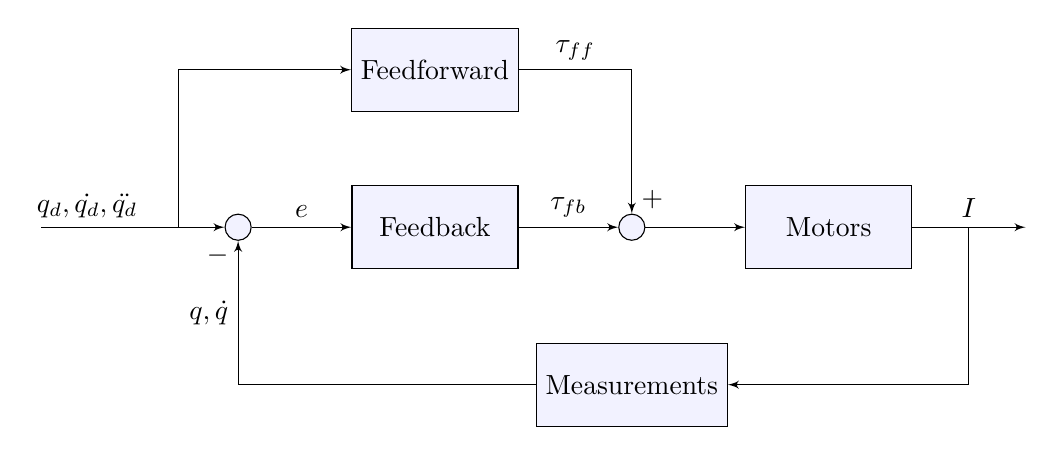
\begin{tikzpicture}[auto,node distance=2.5cm,>=latex']
% placing nodes
\node [input](input){};
\node [sum, right of=input](sum1){};
\node [block, right of=sum1](feedback){Feedback};
\node [block, above of=feedback, node distance=2cm](feedforward){Feedforward};
\node [sum, right of=feedback](sum2){};
\node [block, right of=sum2](motors){Motors};
\node [output, right of=motors](output){};
\node [block, below of=sum2, node distance=2cm](measurements){Measurements};
% connecting nodes
\draw [->](input) -- node[near start]{$q_d,\dot{q_d},\ddot{q_d}$} node[name=in,near end,below]{}(sum1);
\draw [->](in) |- (feedforward);
\draw [->](feedforward) -| node[near start]{$\tau_{ff}$} node[pos=0.95]{$+$}(sum2);
\draw [->](sum1) -- node{$e$} (feedback);
\draw [->](feedback) -- node{$\tau_{fb}$}(sum2);
\draw [->](sum2) -- (motors);
\draw [->](motors) -- node[name=I]{$I$}(output);
\draw [->](I) |- (measurements);
\draw [->](measurements) -| node[pos=0.95]{$-$} node[near end]{$q,\dot{q}$}(sum1); 
\end{tikzpicture}
\caption[Control scheme for Computed Torque controller.]{Control scheme for Computed Torque controller. $I$ is the vector of output current measured from joint actuators which is then transduced to joint positions and velocity.}
\label{fig:computedtorque}
\end{figure}

%%%%%%%%%%%%%%%%%%%%%%%%%%%%%%%%%%%%%%%%%%%%%%%%%%%%%%%%
\paragraph{Inverse Kinematics-based Controller}
Given an end-effector position and orientation, the problem of inverse kinematics consists in determining the corresponding joint configurations. Since the system to solve is in general nonlinear, it's not possible to compute a solution in closed-form. This leads to different scenarios, i.e.\ no admissible solutions in presence of structure singularities, multiple or infinite solutions if the robot is redundant (which is the case of KUKA LWR IV, see Section \ref{sec:therobot}). As an extension of the forward and inverse kinematics problem, it is also possible to define a relationship between the end-effector linear and angular velocity and the joint velocities as follows
\begin{equation}
\dot{x} = J\dot{q} \hspace{1cm} q \in \mathbb{R}^n,\,x \in \mathbb{R}^m
\label{eq:diffkinematics}
\end{equation}
representing the \textit{Differential Kinematics} equation. The mapping is described by the \textit{Jacobian} matrix $J \in \mathbb{R}^{m \times n}$ which depends on the robot configuration. Inverting \eqref{eq:diffkinematics}, leads to the \textit{Inverse Differential Kinematics} problem
\begin{equation}
\dot{q} = J^+\dot{x}
\end{equation}
where $J^+$ is a generalized inverse of the Jacobian. For the project's purpose, it has been implemented in ROS as the Moore-Penrose damped pseudo-inverse through the SVD method, denoted in the sequel as $J^{\dagger}$.\\
In view of the operational space formulation, given a desired end-effector pose $x_d$ and velocity $\dot{x}_d$, a task can be defined as 
\begin{equation}
e = x_d - x(t)
\end{equation}
where $x(t)$ is the end-effector pose at time t.
The related reference motion in the task space is
\begin{equation}
\dot{e}^* = \dot{x}_d + K(x_d - x) = \dot{x}_d + Ke
\end{equation}
where $K$ is a positive definite gain matrix (usually diagonal).

\begin{figure}[h]
\centering
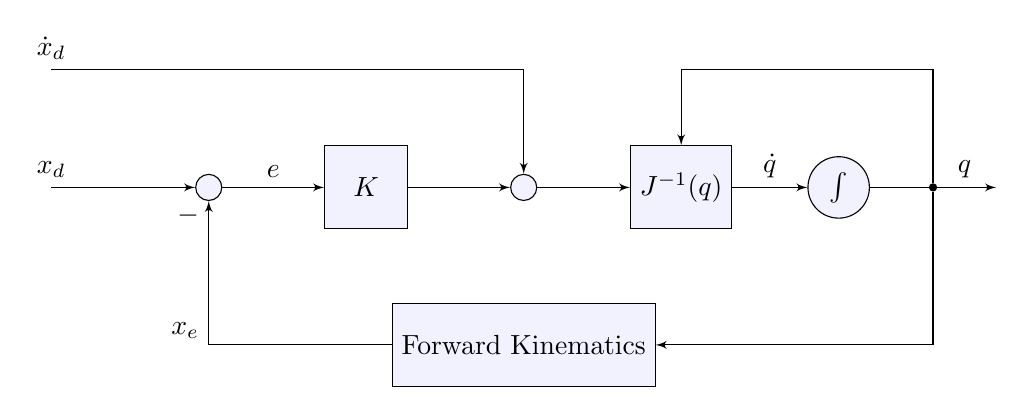
\begin{tikzpicture}[auto,node distance=2cm,>=latex']
% placing nodes
\node [input](input1){};
\node [input, above of=input1, node distance=1.5cm](input2){};
\node [sum, right of=input1](sum1){};
\node [block_small, right of=sum1](K){$K$};
\node [sum, right of=K](sum2){};
\node [block_small, right of=sum2](jac_inv){$J^{-1}(q)$};
\node [sum, right of=jac_inv](integral){$\int$};
\node [output, right of=integral](output){};
\node [block, below of=sum2](forw_kin){Forward Kinematics};
\coordinate [above of=integral,node distance=1.5cm](tmp);
%% connecting nodes
\draw [->](input1) -- node[pos=0]{$x_d$} (sum1);
\draw [->](input2) -| node[pos=0]{$\dot{x}_d$} (sum2);
\draw [->](sum1) -- node{$e$} (K);
\draw [->](K) -- (sum2);
\draw [->](sum2) -- (jac_inv);
\draw [->](jac_inv) -- node{$\dot{q}$} (integral);
\draw [->](integral) -- node[intersection,anchor=base,name=q]{} 
		   node[near end]{$q$} (output);
\draw [->](q) |- (tmp) -| (jac_inv);
\draw [->](q) |- (forw_kin);
\draw [->](forw_kin) -|  node[pos=0.55]{$x_e$} node[pos=0.95]{$-$} (sum1); 
\end{tikzpicture}

\caption{Control scheme for Differential Inverse Kinematics-based controller.}
\label{fig:diffinversekinematics}
\end{figure}

%%%%%%%%%%%%%%%%%%%%%%%%%%%%%%%%%%%%%%%%%%%%%%%%%%%%%%%%
\paragraph{Hierarchical Inverse Kinematics Controller}
It is possible to exploit the redundancy of the manipulator, i.e.\ when the rank of $J$ is smaller than $n$, to assign a secondary task by projecting an arbitrary vector on the null-space of the Jacobian, thus not affecting the higher priority task. So, considering two tasks $e_1$ and $e_2$, the following control law will perform exactly $\dot{e}_1^*$ and, if possible, $\dot{e}_2^*$
\begin{equation}
\dot{q} = J_1^{\dagger}\dot{e}_1^* + (J_{2}P_1)^{\dagger}(\dot{e}_2^* - J_{2}J_1^{\dagger}\dot{e}_1^*)
\end{equation}
This method is called \textit{Stack of Tasks} and can be generalized for $k$ tasks, ensuring a correct hierarchy between them \cite{mansardICAR09},\cite{mansardIEEE09}
\begin{equation}
\begin{dcases}
\dot{q}_0 = 0\\
P_0 = I_n\\
\dot{q}_i = \dot{q}_{i-1} + (J_{i}P_{i-1})^{\dagger}(\dot{e}_i^* - J_{i}\dot{q}_{i-1})\\
P_i = P_{i-1} + (J_{i}P_{i-1})^{\dagger}(J_{i}P_{i-1})
\end{dcases}
\end{equation}
where $P_i$ is the projection operator onto the null-space of $J_i$ and the robot joint velocity realizing all the tasks is $\dot{q}=\dot{q}_k$. This way, all the tasks are decoupled from each other and if a task won't be feasible it will be executed only at its best without disturbing the higher priority tasks.

\begin{figure}
\centering
\includegraphics[width=0.9\textwidth]{hik}
\caption{Simulated robot performing two tasks at different priority levels using Hierarchical Inverse Kinematics.}
\end{figure}

\begin{figure}
\centering
\includegraphics[width=\textwidth]{invkin}
\caption{Evolution of the Mean Square Error (MSE) of two tasks controlled through Hierarchical Inverse Kinematics.}
\end{figure}

%%%%%%%%%%%%%%%%%%%%%%%%%%%%%%%%%%%%%%%%%%%%%%%%%%%%%%%%
\paragraph{Inverse Dynamics-based Controller}
The problem of inverse dynamics in the operational space consists in the determination of the joint torques $\tau$ that realizes a specific motion $\ddot{e}^*$ assigned in terms of $\ddot{x}_d,\dot{x}_d,x_d$, the end-effector desired acceleration,velocity and position
\begin{equation}
\ddot{e}^* = \ddot{x}_d + K_d(\dot{x}_d - \dot{x}) + K_p(x_d - x) = 
\ddot{x}_d + K_{d}\dot{e} + K_{p}e
\end{equation}
where $K_p$ and $K_d$ are positive definite diagonal matrices. Recalling the manipulator dynamic model in the compact form \eqref{eq:compactrobotdynamics}, the choice of the \textit{inverse dynamics control}
\begin{equation}
\tau = M(q)y + n(q,\dot{q})
\end{equation}
leads to a double integrators system
\begin{equation*}
\ddot{q} = y
\end{equation*}
where the control $y$ is designed to track the desired motion $\ddot{e}^*$ through the following second-order relationship
\begin{equation}
\ddot{e}^* = J(q)\ddot{q} + \dot{J}(q,\dot{q})\dot{q}
\end{equation}
It is then possible to write, omitting dependencies in $q$ and its derivatives
\begin{equation}
\ddot{e}^* + b = JM^{-1}\tau
\label{eq:tempinvdyn}
\end{equation}
where $b = JM^{-1}n - \dot{J}(q,\dot{q})\dot{q}$.
Defining $\Omega = JM^{-1}J^T$ and $\Lambda = \Omega^{-1}$ and multiplying \eqref{eq:tempinvdyn} by $\Lambda$ leads to
\begin{equation}
\Lambda\ddot{e}^* + {\Lambda}b = \bar{J}^T\tau
\label{eq:temp2invdyn}
\end{equation}
where $\bar{J} = M^{-1}J^T\Lambda$ is the generalized inverse of $J$ weighted by $M^{-1}$. Finally, multiplying \eqref{eq:temp2invdyn} by $J^T$ it is possible to define the control law that realizes the reference motion $\ddot{e}^*$
\begin{equation}
\tau = J^T\Lambda(\ddot{e}^* + b)
\label{eq:onetaskinversedynamics}
\end{equation}

%%%%%%%%%%%%%%%%%%%%%%%%%%%%%%%%%%%%%%%%%%%%55
\paragraph{Hierarchical Inverse Dynamics Controller}
Equation \eqref{eq:onetaskinversedynamics} implements the inverse dynamics control for a single task $e$. As for inverse kinematics, the manipulator redundancy can be exploited also at dynamics level to give the possibility to execute other lower priority tasks, using the \textit{Stack of Tasks} framework (applied to $k$ tasks)
\begin{equation}
\begin{dcases}
\tau_0 = 0\\
{N_0}^T = I_n\\
\tau_i = \tau_{i-1} + {J_i}^T\Lambda_{i\vert i-1}({\ddot{e}_i}^* + b_i - J_{i}M^{-1}\tau_{i-1}) \\
{N_i}^T = {N_{i-1}}^T - {J_i}^T\Lambda_{i\vert i-1}J_{i}M^{-1}
\end{dcases}
\end{equation}
where $\Lambda_{i\vert i-1} = {\Omega_{i\vert i-1}}^{-1}$ and ${\Omega_{i\vert i-1}} = {J_i}^{T}M^{-1}{N_{i-1}}^TJ_i$. The projection operator is ${N_i}^T$ and the control $\tau$ applied to the robot is $\tau_k$.

\begin{figure}
\centering
\includegraphics[width=0.9\textwidth]{hid}
\caption{Simulated robot performing two tasks at different priority levels using Hierarchical Inverse Dynamics.}
\end{figure}

\begin{figure}
\centering
\includegraphics[width=0.9\textwidth]{invdyn}
\caption[Evolution of the Mean Square Error (MSE) of two tasks controlled through Hierarchical Inverse Dynamics.]{Evolution of the Mean Square Error (MSE) of two tasks controlled through Hierarchical Inverse Dynamics. Notice in the zoomed plot how the higher priority task converges to zero faster.}
\end{figure}

%%%%%%%%%%%%%%%%%%%%%%%%%%%%%%%%%%%%%%%%%%%%%%%%%%%%%%%%%%%%%%%%%%%
\paragraph{Minimum Effort Controller}
Another way to take advantage of the redundant DOFs, other than performing additional motion tasks, is to use the Jacobian null-space projection method to maximize an objective function in the joint space as follows
\begin{equation}
\tau = J^T\Lambda(\ddot{e}^* + b) + N^T\tau_{null}
\label{eq:projectednullspaceobjective}
\end{equation}
where in general $\tau_{null} = \nabla_{q}H(q)$ and $H(q)$ is a differentiable objective funcion to be maximized, implementing a specific criterion with the goal of moving the manipulator in its gradient direction. Taking inspiration from human manipulation, it is possible to reproduce those natural motions in an efficient way, setting the objective function $H(q) = g(q)^{T}Wg(q)$, where $g(q)$ is the gravitational force vector as in \eqref{eq:robotdynamics} and $W$ is a constant diagonal weighting matrix \cite{ajoudani13}. This way, control law \eqref{eq:projectednullspaceobjective} will minimize joint masses and payload gravitational forces while guaranteeing asymptotic stability of the system and not affecting the primary motion task referenced by $\ddot{e}^*$.

\begin{figure}
\centering
\includegraphics[width=0.9\textwidth]{minimumeffort_rviz}
\caption{Simulated robot tracking a circle figure using the Minimum Effort Controller.}
\end{figure}

\begin{figure}
	\centering
	\begin{subfigure}[t]{0.9\textwidth}
		\includegraphics[width=\textwidth]{minimumeffort_X}
		\subcaption{X-Axis}
	\end{subfigure}
	\begin{subfigure}[t]{0.9\textwidth}
		\includegraphics[width=\textwidth]{minimumeffort_Y}
		\subcaption{Y-Axis}
	\end{subfigure}
	\begin{subfigure}[t]{0.9\textwidth}
		\includegraphics[width=\textwidth]{minimumeffort_Z}
		\subcaption{Z-Axis}
	\end{subfigure}
	\caption{Axis-specific end-effector trajectories tracking a circle figure using Minimum Effort Control.}
\end{figure}

%%%%%%%%%%%%%%%%%%%%%%%%%%%%%%%%%%%%%%%%%%%%%%%%%%%%%%%%
\paragraph{Backstep Controller}
Backstepping is a recursive methodology for designing both feedback control laws and associated Lyapunov functions in a systematic way, with the goal of obtaining a good flexibility over the nonlinearities. Consider the following nonlinear system in which the origin is an equilibrium
\begin{equation}
\begin{dcases}
\dot{\xi}_1 = f(\xi_1) + g(\xi_1)\xi_2 \\
\dot{\xi}_2 = h(\xi_1,\xi_2) + \ell(\xi_1,\xi_2)u
\end{dcases}
\label{eq:backsteppingsystem}
\end{equation}
with $\xi_1\in\mathbb{R}^{n_1}, \xi_2\in\mathbb{R}^{n_2},u\in\mathbb{R}^{n_2}$ and $\ell(\xi_1,\xi_2)\in\mathbb{R}^{n_2 \times n_2}$ is invertible for all $\xi_1,\xi_2$. Assume that a stabilizing feedback law $u'=\Gamma(\xi_1)$ exists for the subsystem 
\begin{equation}
\dot{\xi}_1 = f(\xi_1) + g(\xi_1)u'
\end{equation}
and that a Lyapunov function $V(\xi_1)$ is postulated such that
\begin{equation}
\dot{V}(\xi_1) = V_{\xi_1}(f + g\Gamma)
\end{equation}
is at least negative semi-definite, with $V_{\xi_1} = \frac{\partial{V}}{\partial{\xi_1}}$. So, the control of the whole system \eqref{eq:backsteppingsystem} is obtained making $\xi_2$ to track the value of $u'=\Gamma(\xi_1)$.

\begin{figure}[H]
	\centering
	\includegraphics[width=0.9\textwidth]{backstepping_rviz}
	\caption{Simulated robot tracking a 8 figure using Backstepping Control.}
\end{figure}

The backstepping control method can be applied to a robotic manipulator described by its dynamic model \eqref{eq:robotdynamics}, designing the joint torques $\tau$ that track the trajectory $q_d(t)$. Defining the tracking error $e=q-q_d$ and its derivative $\dot{e}=w$, it is possible to consider the following system
\begin{equation}
\begin{dcases}
\dot{e} = w\\
\dot{w} = \ddot{q}-\ddot{q}_d = -\ddot{q}_d - M^{-1}\left(C\dot{q}+g(q)\right) + M^{-1}\tau
\end{dcases}
\label{eq:lagrangianbackstepping}
\end{equation}
which can be interpreted in the form of \eqref{eq:backsteppingsystem}, imposing $e=\xi_1, w=\xi_2, f(e)=0, g(e)=1, \ell(e,t)=M(e+q_d)^{-1}$ and $h(e,w,t)=-\ddot{q}_d(t)-M^{-1}\left(C(\dot{e}+\dot{q}_d)+g\right)$. After performing a stability study with Lyapunov control functions, the backstepping control law for a fully actuated manipulator can be defined as
\begin{equation}
\tau = M\ddot{q}_r + C\dot{q}_r + g(q) - K_{d}s - e
\label{eq:backsteppingcontrollaw}
\end{equation}
where
\begin{align*}
s &= \dot{e} + \Lambda{e}\\
&= \dot{q} - (\dot{q}_d - \Lambda{e}) = \dot{q} - \dot{q}_r
\end{align*}
and $\dot{q}_r$ is the so-called reference velocity. 

\begin{figure}
	\centering
	\begin{subfigure}[t]{0.9\textwidth}
		\centering
		\includegraphics[width=\textwidth]{backstepping_X}
		\subcaption{X-Axis}
	\end{subfigure}
	\begin{subfigure}[t]{0.9\textwidth}
		\centering
		\includegraphics[width=\textwidth]{backstepping_Y}
		\subcaption{Y-Axis}
	\end{subfigure}
	\begin{subfigure}[t]{0.9\textwidth}
		\centering
		\includegraphics[width=\textwidth]{backstepping_Z}
		\subcaption{Z-Axis}
	\end{subfigure}
	\caption{Axis-specific end-effector trajectories tracking a 8 figure using Backstepping Control.}
\end{figure}

%%%%%%%%%%%%%%%%%%%%%%%%%%%%%%%%%%%%%%%%%%%%%%%%%%%%%%%%
\paragraph{Dynamic Sliding PID Controller}
Regarding simple tasks such as set-point regulation, a proportional-integral-derivative (PID) controller would be enough, but the limitation of this class of controllers is that they can't achieve asymptotic stability for trajectory tracking. However, it is possible to enhance PID controllers by applying to them the sliding mode theory, as explained in the sequel \cite{parravega03}. So, given a desired motion specified by $q_d,\dot{q}_d,\ddot{q}_d\in\mathbb{R}^n$, it is analyzed the problem of designing the controller $\tau$ which guarantees the tracking of $q_d(t)$ without any knowledge of the system dynamic model and without introducing high-frequency components, by considering the following steps
\begin{align}
&\dot{q}_r = \dot{q}_d - \alpha\Delta{q} + S_d - \gamma\sigma \label{eq:sliding_qdotref}\\
&\dot{\sigma} = sgn(S_q)
\end{align}
where $\Delta{q}$ is the tracking error $q-q_d$, $\alpha,\gamma\in\mathbb{R}^{n \times n}$ are diagonal positive definite gain matrices and $sgn(S_q)$ represents the input-wise discontinuous signum function of $S_q\in\mathbb{R}^n$, the so-called sliding surface, being defined by
\begin{align}
&S_q = S - S_d\\
&S = \Delta{\dot{q}} + \alpha\Delta{q}\\
&S_d = S(t_0)e^{-\kappa(t-t_0)}
\end{align}
with $\kappa > 0$.
Considering a new error coordinates $S_r$ defined as
\begin{equation}
S_r = \dot{q} - \dot{q}_r
\end{equation}
and substituting $\dot{q}_r$ as in \eqref{eq:sliding_qdotref}, it leads to
\begin{equation}
S_r = S_q + \gamma\sigma
\end{equation}
Finally, the controller $\tau$ which realizes the tracking of $q_d(t)$ in closed loop is
\begin{equation}
\tau = -K_{d}S_r
\end{equation}
where $K_d\in\mathbb{R}^{n \times n}$ is a diagonal symmetric positive definite matrix. According to the controller structure, the semi-global exponential tracking is assured and the passivity of the system is preserved, as long as $\gamma$ in \eqref{eq:sliding_qdotref} and $K_d$ are large enough, for small initial conditions.

\begin{figure}[H]
	\centering
	\begin{subfigure}[t]{0.9\textwidth}
		\centering
		\includegraphics[width=\textwidth]{slidingmode_j1}
		\subcaption{Joint 1}
	\end{subfigure}
	\begin{subfigure}[t]{0.9\textwidth}
		\centering
		\includegraphics[width=\textwidth]{slidingmode_j3}
		\subcaption{Joint 3}
	\end{subfigure}
	\caption{Joint-specific sine waves trajectories tracking using Dynamic Sliding PID Control.}
\end{figure}

\subsubsection{Joint state estimation}

One issue found during the implementation of controllers is the absence of joint velocity values. While the simulated hardware interface takes the joint velocity from simulation, the KUKA LWR arm is equipped with position and torque sensors. Thus, the need to derive the velocities from the position values through a process of online differentiation is prominent. The following methods were visited.

\paragraph{Levant Robust Differentiator}
This method is based on the sliding mode theory and gives asymptotically exact derivatives~\cite{levant06}. In comparison with the Euler method, Levant differentiator performs significantly better in terms of noise rejection and derivation of signals, but the major flaw which led this method to be discarded is that introduces a relevant phase shift. 
\paragraph{Euler method}
This is one of the most basic techniques to compute numerical differentiation and follows the equation
\begin{equation}
\dot{q}_n = \frac{q_n - q_{n-1}}{h},
\end{equation}
where $h$ is the sampling time. Since the output of this differentiator is usually noisy, typically, a exponential smoothing filter is used as the post-process signal processing as
\begin{equation}
\tilde{\dot{q}}_n = \alpha\dot{q}_n + (1-\alpha)\tilde{\dot{q}}_{n-1},
\end{equation}
where $\tilde{\dot{q}}$ denotes the smoothed value and $\alpha\in(0,1)$ is the smoothing factor. This is the current joint state estimation method for the arm.
%So, according to the tests conducted and evaluating a trade-off between exact but out-of-phase signals and noisy but coherent signals, the best method resulted the Euler one.

% %%%%%%%%%%%%%%%%%%%%%%%%%%%%%%%%%%%%%%%%%%%%%%%%%%%%%%%%
% %%%%%%%%%%%%%%%%%%%%%%%%%%%%%%%%%%%%%%%%%%%%%%%%%%%%%%%%
% %%%%%%%%%%%%%%%%%%%%%%%%%%%%%%%%%%%%%%%%%%%%%%%%%%%%%%%%
% \subsubsection{Controller design issues}
% During the process of controllers design, certainly one requirement that has to be met is to reach an efficient complexity in terms of computational resources. In the sequel it's analyzed a category of control strategies which requires, at least in this case study, the exploitation of a big amount of resources that unfortunately weren't available on the machines used for experiments.

% %%%%%%%%%%%%%%%%%%%%%%%%%%%%%%%%%%%%%%%%%%%%
% \paragraph{Adaptive Control}
% In this section it has been assumed that the dynamic model of the robot is perfectly known at any instant of time, but, in practice, this can't be always true. In fact there exist some model uncertainties depending on the robot configuration, mainly mechanical parameters like inertia matrices and masses for the single links or those related to the robot payload. To overcome this intrinsic problem, it is always possible to write the dynamic model of the robot \eqref{eq:robotdynamics} through a linear parametrization
% \begin{equation}
% M(q)\ddot{q} + C(q,\dot{q})\dot{q} + g(q) = Y(q,\dot{q},\ddot{q})\pi = \tau
% \end{equation}
% where the vector $\pi\in\mathbb{R}^r$ contains the combinations of the aforementioned physical parameters and $Y(q,\dot{q},\ddot{q})\in\mathbb{R}^{n\times r}$ is called the \textit{regressor} matrix. In brief, this sums up the aim of the \textit{Adaptive Control}, which, as the name suggests, makes the control law to adapt to the variations of the unknown robot model parameters. Recently, an analytic closed formula for the regressor has been derived from the Lagrange equations, in terms of the Denavit-Hartenberg parameters and the joints configurations  $q,\dot{q},\ddot{q}$, and implemented in \textit{Mathematica} environment \cite{gabiccini09}. For a 7-links manipulator like KUKA LWR, the resulting regressor matrix has dimensions $7$x$70$ in its unsimplified form, making literally impossible to handle an adaptive control with the owned instruments.

% %%%%%%%%%%%%%%%%%%%%%%%%%%%%%%%%%%%%%%%%%%%%
% \paragraph{Gravity Compensation}
% Recalling the built-in controllers \eqref{eq:cartesianstiffnesscontroller}, \eqref{eq:axisspecificstiffnesscontroller} of the KUKA LWR arm, the term $f_{dynamics}(q,\dot{q},\ddot{q})$ must be analyzed. It refers to the gravity compensation performed internally by the robot, in a way that the commanded torque isn't indeed affected by the gravitational field. This, unfortunately, generates a conflict between the internal compensation and the whole control law, which at dynamic level requires the knowledge of the gravitational force to compute the input torques. Since such term can't be forced to zero, one workaround could be that of not considering the gravity ($g(q)=0$) in all model-based controller, introducing a really negligible error.
\subsection{Pisa/IIT SoftHand}
\label{sec:softhand}

The Pisa/IIT SoftHand is a 5-finger hand that introduces an implementation of the adaptive synergy transmission~\cite{Catalano2014Adaptive}. Fig~\ref{fig:soft_hand}.

\begin{figure}[b]
\centering
\includegraphics[width=0.4\textwidth]{soft_hand.png}
\caption{The Pisa/IIT SoftHand, 1 motor and 19 dof.}
\label{fig:soft_hand}
\end{figure}

\subsubsection{Hardware interface}

The real hardware interface is implemented using the API provided by qbrobotics$^{\copyright}$~\cite{qbrobotics_software}, using position commands. 

The simulated hardware interface is special. 

The interface is loaded into Gazebo as a plug-in that has access to the simulation, useful to read the full hand state as well as contacts, and receives commands from the controller in position. To simulate the SoftHand behavior the four elements described below are used within the interface implementation.

\paragraph{Joint description} The knuckle joint for all fingers is a regular revolute joint, so they are specified as such using common URDF tags~\ref{webros}. The inter-phalangeal joints, however, are based compliant rolling-contact joints, which are not among the library of joint types in any of the simulation environments available today, as far as the authors know. Thus, it requires a special treatment to emulate the kinematic motion resulting from rolling. To this end, each inter-phalangeal joint is the combination of two revolute joints having the same angle, that is, coupled with the same ratio to the reduced synergy actuator. For more details on this, see the preliminary work of modeling the Pisa/IIT SoftHand in ADAMS (in Italian, but the subject can be followed readily)~\cite{Piazza2013Studio}, available at~\href{./attachedPapers/CristinaPiazzaReport.pdf}{this link}.

\paragraph{Transmission interface} This part contains the mapping between the actuator (one motor) and joints (19 revolute joints and 19 mimic joints) in position and effort domains. That is, according to~\cite{Catalano2014Adaptive}, actuating the adaptive synergistic hand by direct control of the reduced synergy vector $\sigma^{1}$, leads to the system
\begin{equation}
\left[ \begin{array}{cc} -E & R^{T} \\ R & 0 \end{array} \right] \left[ \begin{array}{c} q \\ R  \end{array} \right] = \left[ \begin{array}{c} J^{T}f_{c} \\ \sigma^{1}  \end{array} \right],
\end{equation}
where $E$ is the joint space stiffness matrix, $R$ is the transmission ratio matrix, $q$ the reference position of the springs in the phalanges, $J$ is the grasp Jacobian and $f_c$ is the wrench associated with the contact forces. The solution to this system was implemented for the different mappings between actuator and joints.

\paragraph{Contact wrenches $f_c$} An out-of-the-box Gazebo plug-in is available that is loaded per each body, i.e. each phalanx, that provides all contact point and wrenches, as well as the resultant wrench at the body reference frame. The later is particularly useful for the next element.

\paragraph{Grasp Jacobian $J$} A kinematic library is used to obtained all Jacobian's that relate all phalanges to the different finger sub-chains. That is, for one finger with 4 joints, 4 Jacobian's are computed at the current hand joint state, namely, the consideration of 4, 3, 2, and 1 joints, respectively. Since the total contact wrench per phalanx is already expressed in the phalanx reference frame, the Jacobian's are obtained using that as the reference frame, and the palm as the base frame. 

To illustrate the implementation, Fig.~\ref{fig:soft_hand_gazebo} shows the hand prior to closing and after closing, with an obstacle in the middle. Recall that the only actuation is the synergy motor, and the rest of joints are commanded through the implementation of the adaptive synergy transmission as described above.

\begin{figure}
\centering
\includegraphics[width=0.45\textwidth]{open.png}
\hspace{1pt}
\includegraphics[width=0.45\textwidth]{close.png}
\caption{The Pisa/IIT SoftHand simulated in Gazebo at full open (left) and close (right) commanded configurations.}
\label{fig:soft_hand_gazebo}
\end{figure}

\subsubsection{Joint state estimation}

At this point, there are two on going works regarding this issue that we expect to converge in a sensor fusion approach during the time remaining on the project. The first one is presented in DR 3.1, where an IMU-based glove provides an accurate estimate of the joint angles. The second approach is a simulator-in-the-loop extended Kalman filter, where the simulation play the role of the system model to give the estimated joint values, and motor position (via a position encoder) and effort (estimated from the current measurement) are used as measurements to update the filter via the adaptive synergy transmission equations implemented in the transmission interface as described above. This work is being submitted to IROS 2015, for more details see the attached at~\href{}{this link}.
\subsection{Software: KIT Head package}
\label{sec:kithead}

The Karlsruhe humanoid head~\cite{Asfour2008KITHead} was acquired as the testbed for active gaze strategies. Fig.~\ref{fig:kit_head} shows a picture of the real device.

\begin{figure}
\centering
\includegraphics[width=0.25\textwidth]{kithead.png}
\caption{The Karlsruhe humanoid head.}
\label{fig:kit_head}
\end{figure}

\subsubsection{Hardware interface}

The real hardware interface is still under development. The simulated hardware interface considers the default behavior of a robot using position controlled motors. This is good enough for the planning and simulation environment, specially to test active gaze control. In order to do that, we added the simulation of point cloud acquisition, as well as two RGB cameras per eye to be as close as possible to what the KIT head offers. The simulation of the cameras is described next.

\subsubsection{Camera simulation}
There are out-of-the-box camera plug-ins for both kind of cameras, RGB and RGB-D. Both are used in the simulated head. The point cloud and images are published in an uncalibrated frame as well as in the real robot could be. Real calibration values can be loaded to have camera and robot  under the same tree of connectivity. Parameters such as noise and noise type can be set to test active gaze control and object recognition in ideal and not so ideal conditions. Fig.~\ref{fig:kit_vision} shows the simulated RGB and RGB-D cameras mounted on the eyes and forehead. Note that, the robot model has been set to almost transparent in the visualizer at the bottom, and the point cloud is overlaid covering the hand and wrist.

\begin{figure}[h!]
\centering
\includegraphics[width=0.7\textwidth]{headVision.png}
\caption{Simulation of RGB (top) and RGB-D (bottom) cameras available in the KIT head.}
\label{fig:kit_vision}
\end{figure}
%!TEX root = MS42.tex
\section{Conclusions and Future Works}
The present work had the aim of implementing an extended set of different classes of controllers for the robotic arm KUKA LWR IV, exploiting a flexible system which is rapidly growing in the field of robotics, including research and whole industrial processes. In fact, all the code produced could not only be accessed and used from users operating the same robot, but ideally from everyone who works with ROS, at least performing some minor edits to fit their needs. Thinking about future works starting from this project, it could be interesting the extension to a bimanual system in a human-like arms configuration. For example, taking advantage of the Stack of Tasks framework could be also provided obstacle and collision avoidance, making easier the interaction between the robot and humans or the handling of more complex operations. 
\newpage

\subsection{Technical report: Studio e simulazione in ambiente Adams della Pisa-IIT Softhand - Cap. 2 and 3 } \label{sec:AdamsSoftHand}
This report is written in Italian, but still figures and equations can be followed readily. It concerns an excerpt of the implementation of the Pisa/IIT SoftHand mechanism in the Adams\copyright, developed as part of requirements to approve one of the classes imparted by Prof. Marco Gabiccini.
\includepdf[pages=5-26]{./attachedPapers/CristinaPiazzaReport.pdf}

\end{document}
